\documentclass[11pt]{article}
\usepackage[margin=1in]{geometry}
\usepackage[T1]{fontenc}
\usepackage{lmodern,microtype}
\usepackage{amsmath,amssymb,amsthm,mathtools}
\usepackage{graphicx,booktabs,xcolor,xurl,hyperref}
\hypersetup{colorlinks=true,linkcolor=blue!45!black,citecolor=blue!45!black,urlcolor=blue!45!black}
\newtheorem{theorem}{Theorem}[section]
\newtheorem{lemma}[theorem]{Lemma}
\newtheorem{corollary}[theorem]{Corollary}
\newtheorem{proposition}[theorem]{Proposition}
\theoremstyle{remark}\newtheorem{remark}[theorem]{Remark}
\newcommand{\R}{\mathbb R}
\newcommand{\N}{\mathbb N}
\newcommand{\Z}{\mathbb Z}
\newcommand{\T}{\mathbb T}
\newcommand{\dd}{\,\mathrm d}
\newcommand{\supp}{\operatorname{supp}}
\newcommand{\diam}{\operatorname{diam}}
\newcommand{\Impart}{\operatorname{Im}}
\newcommand{\pos}[1]{(#1)_+}
\newcommand{\norm}[1]{\left\lVert#1\right\rVert}
\title{Sharp reciprocal-zero inequalities for positive Fourier filters\\
\large Support uncertainty, stability, and square-frequency gaps}
\author{Research manuscript}
\date{27 November 2026}

\begin{document}
\maketitle
\begin{abstract}
Let $\mu$ be a probability measure supported in an interval of length $L$, and let
$\lambda_j>0$ be the imaginary parts of selected upper-half-plane zeros of
$G(z)=\int e^{zt}\dd\mu(t)$, counted with their actual multiplicities.
We prove the sharp finite inequalities
$\sum_{j=1}^n\lambda_j^{-p}\le (L/\pi)^p\sum_{j=1}^n(2j-1)^{-p}$ for every $p>0$.
In particular, the full reciprocal-square sum is at most $L^2/8$.
All equality cases are two-point endpoint measures; for zeros on the imaginary
axis their endpoint masses are equal. A quantitative stability theorem controls
the distance to this equal-mass measure by the square root of the moment deficit.
The proof combines the ProveIt project's strip identity and mean-frequency bound
with a partial-sum majorization argument, and is reproduced in full.
It gives an affirmative answer, with optimal constant, to the square-sum support
inequality in Steinerberger's question ``A kind of uncertainty principle?''
Convex separation also gives sharp-order lower bounds for zero-free intervals of
trigonometric polynomials with square frequencies, answering the order-of-magnitude
alternative in Question 2 of Kozma--Oravecz. The exact wide-band extremum is not
determined. Every result in this manuscript is unconditional.
\end{abstract}

\section{Results, provenance, and scope}

We use the angular Fourier convention
\[
 \widehat\mu(\lambda)=\int_\R e^{i\lambda t}\dd\mu(t).
\]
Unless stated otherwise, $\mu$ is a compactly supported probability measure,
$L=\diam(\supp\mu)>0$, and $G(z)=\int e^{zt}\dd\mu(t)$.
The word ``selected'' permits any submultiset of the zero divisor: a zero may be
repeated no more often than its analytic multiplicity. Distinct complex zeros
may have the same imaginary part.

\begin{theorem}[Sharp reciprocal moments]\label{thm:main}
Let $n\ge1$ and let $\rho_1,\ldots,\rho_n$ be selected zeros of $G$ with
$0<\lambda_1\le\cdots\le\lambda_n$, where $\lambda_j=\Impart\rho_j$.
For every real $p>0$,
\begin{equation}\label{eq:finite}
 \sum_{j=1}^n\lambda_j^{-p}
 \le \left(\frac L\pi\right)^p
       \sum_{j=1}^n\frac1{(2j-1)^p}.
\end{equation}
Equality holds if and only if, for some $u\in\R$ and $0<b<1$,
\begin{equation}\label{eq:extreme}
 \mu=b\delta_u+(1-b)\delta_{u+L},\qquad
 \rho_j=\frac1L\log\frac b{1-b}+\frac{(2j-1)\pi i}{L}
 \quad(1\le j\le n).
\end{equation}
If all selected zeros are Fourier zeros, so $\rho_j=i\lambda_j$, equality requires
$b=1/2$.

For an arbitrary finite or infinite selected zero multiset and $p>1$,
\begin{equation}\label{eq:infinite}
 \sum_j\lambda_j^{-p}
 \le\left(\frac L\pi\right)^p(1-2^{-p})\zeta(p).
\end{equation}
Equality in \eqref{eq:infinite} holds precisely for \eqref{eq:extreme} with all
$j\ge1$. In particular,
\begin{equation}\label{eq:square}
 \boxed{\displaystyle\sum_j\frac1{(\Impart\rho_j)^2}\le\frac{L^2}{8}.}
\end{equation}
\end{theorem}

The finite constants in \eqref{eq:finite} are attained; they do not arise merely
as limits. The theorem bounds zero heights without placing any restriction on
their real parts. That strengthening is useful because a positive measure need
not have any zeros on the imaginary axis.

The starting point is the strip identity and mean-frequency theorem in
\path{Article/sections/fil.tex} of the ProveIt repository \cite{ProveIt}, at the
fixed revision recorded below. We retain their attribution and reproduce the
analytic details. The strip identity is an exponential-sum analogue of the
integrated Obrechkoff inequality of Eremenko--Fryntov \cite{EF}. The passage from
partial sums to decreasing convex functions is standard majorization, here
written as an elementary integral argument.

The extensions developed in this manuscript are the sharp reciprocal-moment
family for arbitrary complex zero heights, its full equality and Fourier
stability statements, and the applications to the two named questions. These
statements were not located in the inspected repository article or its sixteen
incoming research archives. Targeted searches did not locate an earlier statement
of the sharp support inequality proved here. This records the scope of the
comparison, rather than certifying publication priority.

The repository originates in work on RH and Dirichlet GRH. None of its RH or GRH
assertions is an assumption of this manuscript: the positive-measure argument
below is self-contained. In particular this paper does not require an assessment
of the repository's complete formalization or of broader nonabelian GRH claims.

\section{The strip identity and finite moment reduction}

\begin{lemma}[Integrated strip identity]\label{lem:strip}
Let
\[
 G(z)=\sum_{j=0}^M w_j e^{t_jz},\qquad
 0=t_0<t_1<\cdots<t_M=L,\quad w_j>0,\quad\sum_jw_j=1.
\]
For every $T\ge0$,
\begin{equation}\label{eq:strip}
 J(T):=\int_\R\bigl(\log G(x)-\log|G(x+iT)|\bigr)\dd x
 =\frac{LT^2}{2}-2\pi\sum_{\substack{G(\rho)=0\\0<\Impart\rho<T}}
       (T-\Impart\rho)\ge0.
\end{equation}
Zeros are counted with multiplicity. Boundary zeros at height $T$ may be included
with zero contribution.
\end{lemma}

\begin{proof}
For real $x$, $G(x)>0$ and $|G(x+iy)|\le G(x)$. The integrand in
\eqref{eq:strip} is therefore nonnegative. At the right endpoint,
\[
 G(x+iy)=w_Me^{L(x+iy)}\bigl(1+O(e^{-(L-t_{M-1})x})\bigr)
 \quad(x\longrightarrow+\infty),
\]
uniformly in $y$. There is an analogous left-end expansion
$G(x+iy)=w_0(1+O(e^{t_1x}))$ as $x\to-\infty$.
Thus all zeros lie in a fixed vertical strip, and the integrand has integrable
exponential tails uniformly in $y$. There are finitely many zeros in every
bounded horizontal strip. At a zero of order $k$, local factorization writes
$\log|G(z)|=k\log|z-\rho|+v(z)$ with $v$ harmonic. These logarithmic
singularities are integrable on horizontal lines. They also show that $J$ is
continuous at heights of zeros.

Put $u(x,y)=\log|G(x+iy)|$. As distributions,
\[
 u_{xx}+u_{yy}=2\pi\sum_{G(\rho)=0}\operatorname{ord}_\rho(G)\,\delta_\rho.
\]
Integrate first in $x$ with cutoffs beyond the zero-containing strip and then
send the cutoffs to infinity. The endpoint expansions give
$u_x(+\infty,y)=L$ and $u_x(-\infty,y)=0$. Consequently
\[
 J''(y)=L-2\pi\sum_{G(\rho)=0}
            \operatorname{ord}_\rho(G)\,\delta_{\Impart\rho}(y).
\]
There are no zeros on the real axis. Also $J(0)=0$, and conjugation gives
$J(-y)=J(y)$, hence $J'(0)=0$. Integrating twice on $[0,T]$ gives
\eqref{eq:strip}. Continuity handles heights containing boundary zeros.
\end{proof}

\begin{lemma}[Finite preservation of prescribed zeros]\label{lem:finite}
Given any finite selected multiset of zeros of the Laplace transform of a compactly
supported probability measure, there is a finitely supported probability measure
on the same supporting interval whose transform has every selected zero to at
least the prescribed order.
\end{lemma}

\begin{proof}
For each distinct prescribed zero $\rho$ of selected order $k$, take the real
and imaginary parts of $t^\ell e^{\rho t}$ for $0\le\ell<k$. These finitely
many continuous functions define a vector-valued map on the compact support of
$\mu$. Its integral is the zero vector. This vector lies in the compact convex
hull of the image. Carath\'eodory's theorem expresses it as a convex combination
of at most one more than the dimension many image points. The resulting atomic
probability preserves all the derivative equations. Its support diameter is
no larger than the original one.
\end{proof}

\begin{proposition}[Prefix-sum bound]\label{prop:prefix}
For selected upper-half-plane zeros of $G$, ordered by heights
$0<\lambda_1\le\cdots\le\lambda_n$, one has
\begin{equation}\label{eq:prefix}
 S_m:=\sum_{j=1}^m\lambda_j\ge\frac{\pi m^2}{L}
 \qquad(1\le m\le n).
\end{equation}
\end{proposition}

\begin{proof}
Fix a prefix of length $m$. By Lemma~\ref{lem:finite}, replace $\mu$ by an
atomic probability preserving these zeros. Translate its left endpoint to zero
and let its diameter be $D\le L$. A one-point measure has no zeros, so $D>0$.
Let $\kappa=S_m/m$ and apply Lemma~\ref{lem:strip} with $T=2\kappa$.
The contribution of the selected zeros to the strip sum is at least
\[
 \sum_{j=1}^m\pos{T-\lambda_j}
 \ge mT-S_m=m\kappa.
\]
Other zeros only increase that sum. Hence
$0\le J(T)\le2D\kappa^2-2\pi m\kappa$, giving
$S_m\ge\pi m^2/D\ge\pi m^2/L$.
\end{proof}

This also proves local finiteness of the projected zero divisor without any
endpoint-atom assumption on the original measure: if $m$ selected zeros have
heights at most $T$, then $\pi m^2/L\le mT$, so $m\le LT/\pi$.
Thus infinitely many zeros cannot accumulate at a bounded positive height,
even by escaping in the real direction.

\section{Majorization, sharpness, and other convex statistics}

\begin{lemma}[Hinge domination]\label{lem:hinge}
Let $c=\pi/L$ and $v_j=c(2j-1)$. For a selected list of $n$ zero heights, put
\[
 H_\lambda(t)=\sum_{j=1}^n\pos{t-\lambda_j},\qquad
 H_v(t)=\sum_{j=1}^n\pos{t-v_j}.
\]
Then $H_\lambda(t)\le H_v(t)$ for all real $t$.
\end{lemma}

\begin{proof}
For any sorted list, with $S_0=0$,
\[
 H_\lambda(t)=\max_{0\le m\le n}(mt-S_m).
\]
Indeed the maximizing prefix consists of the entries below $t$, with ties
irrelevant. Proposition~\ref{prop:prefix} gives $S_m\ge cm^2$.
Since $\sum_{j=1}^m v_j=cm^2$, the same formula for the odd list proves the claim.
\end{proof}

\begin{proof}[Proof of Theorem~\ref{thm:main}]
For $x>0$ and $p>0$, direct integration gives
\begin{equation}\label{eq:hinge-integral}
 x^{-p}=p(p+1)\int_0^\infty\pos{t-x}t^{-p-2}\dd t.
\end{equation}
Integrating Lemma~\ref{lem:hinge} against the positive weight in
\eqref{eq:hinge-integral} proves \eqref{eq:finite}.

If equality holds, the continuous nonnegative function $H_v-H_\lambda$ has
zero integral against a strictly positive weight. It vanishes identically.
Its derivative jumps recover the two multisets, so
$\lambda_j=(2j-1)\pi/L$. In particular there is a zero
$\rho=\beta+i\pi/L$. Translate the support to $[0,L]$. The imaginary part of
$G(\rho)=0$ is
\[
 \int_0^L e^{\beta t}\sin(\pi t/L)\dd\mu(t)=0.
\]
The integrand is positive in $(0,L)$ and zero at the endpoints. Thus $\mu$ is
supported on the two endpoints. Both endpoint masses are nonzero because its
diameter is $L$. Writing them as $b,1-b$, the real equation gives
$e^{\beta L}=b/(1-b)$. The transform's zeros are exactly those in
\eqref{eq:extreme}. Conversely that measure realizes the indicated zeros and
attains the bound. The Fourier specialization has $\beta=0$, hence $b=1/2$.

For an infinite multiset, local finiteness permits increasing enumeration.
Apply \eqref{eq:finite} to every finite prefix and use monotone convergence to
get \eqref{eq:infinite}. For its equality statement, use the locally finite
infinite hinge functions. Lemma~\ref{lem:hinge}, now with a supremum over all
$m\ge0$, still holds. Tonelli's theorem and \eqref{eq:hinge-integral} show
that equality forces equality of the infinite hinges. Thus all odd heights
occur and the preceding endpoint argument applies. Finally
$(1-2^{-2})\zeta(2)=\pi^2/8$ gives \eqref{eq:square}.
\end{proof}

\begin{corollary}[Decreasing convex statistics]\label{cor:convex}
Suppose $f:(0,\infty)\to[0,\infty)$ is twice continuously differentiable,
decreasing and convex, and $f(t)\to0$ as $t\to\infty$. Then
\[
 \sum_{j=1}^n f(\lambda_j)\le
 \sum_{j=1}^n f\!\left(\frac{(2j-1)\pi}{L}\right).
\]
The infinite analogue holds whenever the right side is finite. In particular,
for any selected finite or infinite multiset,
\begin{align}
 \sum_j e^{-s\lambda_j}&\le\frac1{2\sinh(\pi s/L)}&& (s>0),\label{eq:heat}\\
 \prod_j\left(1+\frac{x^2}{\lambda_j^2}\right)&\le\cosh(Lx/2)&& (x\ge0).
 \label{eq:product}
\end{align}
Equality in either full bound, for $s>0$ or $x>0$, has the same classification
as equality in \eqref{eq:infinite}.
\end{corollary}

\begin{proof}
Convexity and decay give $f'(t)\to0$ and $t f'(t)\to0$. For example
$0\le-tf'(t)\le2f(t/2)$. Integrating by parts therefore gives
$f(x)=\int_0^\infty\pos{t-x}f''(t)\dd t$.
Use Lemma~\ref{lem:hinge}. For \eqref{eq:heat}, the odd-grid sum is a geometric
series. For \eqref{eq:product}, apply the inequality to
$f(u)=\log(1+x^2/u^2)$, for which
\[
 f''(u)=\frac{2x^2(3u^2+x^2)}{u^2(u^2+x^2)^2}>0\quad(x>0),
\]
and use the Euler product
$\cosh y=\prod_{j\ge1}(1+4y^2/((2j-1)^2\pi^2))$.
The product converges by \eqref{eq:square}. Strict positivity of the relevant
second derivatives proves the equality claim by the hinge argument.
\end{proof}

\section{An optimal answer to the square-sum support question}

We now use $\T=\R/\Z$, with
$\widehat f(a)=\int_\T f(t)e^{-2\pi iat}\dd t$.
The choice of circle normalization matters for the numerical constant.

\begin{theorem}[Sharp support uncertainty]\label{thm:support}
Let $A\subset\N$ be finite and nonempty, $n=|A|$, and let
$f\in L^1(\T)$ be nonnegative with positive integral. Suppose that
$\supp f\subset(-r,r)$ and $\widehat f(a)=0$ for every $a\in A$.
Then
\begin{equation}\label{eq:finite-support}
 r\ge C_n\left(\sum_{a\in A}\frac1{a^2}\right)^{1/2},\qquad
 C_n=\frac1{4\sqrt{\sum_{j=1}^n(2j-1)^{-2}}}.
\end{equation}
In particular,
\begin{equation}\label{eq:support}
 \boxed{\displaystyle r\ge\frac1{\sqrt2\,\pi}
             \left(\sum_{a\in A}\frac1{a^2}\right)^{1/2}.}
\end{equation}
Each $C_n$, as well as the universal constant $1/(\sqrt2\pi)$, is optimal,
even when $f$ is required to be smooth. In that class sharpness is an infimum,
rather than equality by an atomic extremizer.
\end{theorem}

\begin{proof}
First suppose $r<1/2$. Lift $f$ to $(-r,r)\subset\R$ and normalize its integral
to one, obtaining a probability measure of diameter at most $2r$.
Its transform vanishes at the angular frequencies $2\pi a$, $a\in A$.
The case $p=2$ of \eqref{eq:finite} gives
\[
 \frac1{4\pi^2}\sum_{a\in A}a^{-2}
 \le\frac{4r^2}{\pi^2}\sum_{j=1}^n(2j-1)^{-2},
\]
which is \eqref{eq:finite-support}. If $r\ge1/2$, the same inequality is
automatic because its right-side lower bound for $r$ is at most
$\pi/(4\sqrt6)<1/2$. Letting the finite odd sum increase to $\pi^2/8$ gives
\eqref{eq:support}.

For sharpness take $A_n=\{1,3,\ldots,2n-1\}$ and
$\nu=\tfrac12(\delta_{-1/4}+\delta_{1/4})$. Every odd Fourier coefficient of
$\nu$ is zero. Convolve $\nu$ with a smooth nonnegative probability bump supported
in $(-\varepsilon,\varepsilon)$. The resulting smooth nonnegative function
retains those exact zeros and has support contained in
$(-1/4-\varepsilon,1/4+\varepsilon)$. For fixed $n$, letting
$\varepsilon\downarrow0$ gives the best constant $C_n$; then $n\to\infty$
gives $1/(\sqrt2\pi)$. The equality classification of Theorem~\ref{thm:main}
excludes equality by an absolutely continuous measure in the sharp finite
measure bound.
\end{proof}

Steinerberger's \emph{Some Open Problems}, Problem 41 in the indexed
31 March 2026 version, explicitly asks whether a lower bound proportional to
$\bigl(\sum_{a\in A}a^{-2}\bigr)^{1/2}$ holds under these support and positivity
conditions \cite{Steinerberger}. Theorem~\ref{thm:support} answers that inequality
and identifies its best universal constant. It does not give the exact minimum
support radius for every prescribed set $A$.

For the alternative angular circle $\R/(2\pi\Z)$ with Fourier convention
$e^{-iat}$, the radius in \eqref{eq:support} is multiplied by $2\pi$.
The optimal constant is then $\sqrt2$. This prevents a normalization ambiguity
when comparing the statement with a formulation using $\cos(at)$.

\section{Quantitative stability of the Fourier extremizer}

For probability measures on $\R$, $W_1$ denotes the infimum of the expected
transport cost $|x-y|$ over all couplings. In the next theorem the zeros must be
\emph{Fourier zeros}. Arbitrary complex-height extremizers need not have equal
endpoint weights.

\begin{theorem}[A deficit controls transport distance]\label{thm:stability}
Let $\mu$ be supported in $[-L/2,L/2]$, and let $(\lambda_j)$ be a nonempty finite
or infinite selected multiset of positive zeros of $\widehat\mu$. Put
\[
 \Delta=\frac{\pi^2}{8}-\left(\frac\pi L\right)^2
                         \sum_j\lambda_j^{-2},\qquad
 \nu_* =\tfrac12(\delta_{-L/2}+\delta_{L/2}).
\]
If $0\le\Delta\le1/8$, then
\begin{equation}\label{eq:stability}
 W_1(\mu,\nu_*)\le5L\sqrt\Delta.
\end{equation}
No symmetry of $\mu$ is assumed. The constant and the exponent in this stability
bound are not asserted to be optimal.
\end{theorem}

\begin{proof}
Scale the zero heights by $L/\pi$ and let their least value be $a=1+\eta$.
Proposition~\ref{prop:prefix} gives $a\ge1$. The scaled actual hinge vanishes
on $[1,a]$, whereas the full odd-grid hinge is at least $t-1$ there.
By \eqref{eq:hinge-integral},
\begin{equation}\label{eq:deficit-first}
 \Delta\ge6\int_1^a(t-1)t^{-4}\dd t
 =1-\frac3{a^2}+\frac2{a^3}
 =\frac{\eta^2(3+\eta)}{(1+\eta)^3}.
\end{equation}
The expression as a function of $a\ge1$ is increasing and equals $1/2$ at
$a=2$. Thus $\eta<1$. On $0\le\eta\le1$ it is at least $\eta^2/2$, so
\begin{equation}\label{eq:eta}
 0\le\eta\le\sqrt{2\Delta}\le1/2.
\end{equation}

Let $d(x)=L/2-|x|$, the distance to the nearest endpoint. Since
$\int\cos(\lambda_1x)\dd\mu(x)=0$ and cosine is 1-Lipschitz,
\[
 \int\cos(\pi x/L)\dd\mu(x)\le\pi\eta/2.
\]
For $0\le d\le L/2$, $\sin(\pi d/L)\ge2d/L$. Therefore
\begin{equation}\label{eq:mass-core}
 \int d(x)\dd\mu(x)\le\frac{\pi\eta L}{4}.
\end{equation}
Push every point to a nearest endpoint, obtaining
$\nu=b\delta_{L/2}+(1-b)\delta_{-L/2}$. This coupling costs
$E:=\int d\dd\mu$. The imaginary Fourier equation and the
$\lambda_1$-Lipschitz property of sine imply
\[
 |2b-1|\cos(\pi\eta/2)
 =\left|\int\sin(\lambda_1x)\dd\nu(x)\right|
 \le\lambda_1 E.
\]
Moving the excess endpoint mass costs $L|b-1/2|$. The triangle inequality yields
\[
 W_1(\mu,\nu_*)\le
 E\left(1+\frac{\pi(1+\eta)}{2\cos(\pi\eta/2)}\right).
\]
Use \eqref{eq:mass-core} and \eqref{eq:eta}. The coefficient of
$L\sqrt\Delta$ is at most
\[
 \frac{\pi\sqrt2}{4}
 \left(1+\frac{3\pi}{4\cos(\pi/4)}\right)<5,
\]
which proves the result.
\end{proof}

\section{Duality with zero-free intervals}

Let $A\subset\N$ be finite and nonempty. Define $M(A)$ as the supremum of lengths
of intervals on $\R/\Z$ on which some nonzero real trigonometric polynomial
\[
 P(x)=\sum_{a\in A}\bigl(c_a\cos(2\pi ax)+d_a\sin(2\pi ax)\bigr)
\]
has no zero. Coefficients are allowed to vanish: the spectrum is contained in
$\pm A$. Define $B(A)$ as the least support diameter of a probability measure
on $\R$ whose angular Fourier transform vanishes at every $a\in A$.

\begin{proposition}[Exact finite-dimensional duality]\label{prop:duality}
The minimum defining $B(A)$ exists, and
\begin{equation}\label{eq:duality}
 M(A)=\frac{B(A)}{2\pi}.
\end{equation}
If $A=\{a_1<\cdots<a_n\}$, then
\begin{equation}\label{eq:general-gaps}
 \max_{1\le m\le n}\frac{m^2}{2\sum_{j=1}^m a_j}
 \le M(A)\le\frac12\sum_{j=1}^n\frac1{a_j}.
\end{equation}
\end{proposition}

\begin{proof}
A feasible probability exists: convolve the measures
$\tfrac12(\delta_0+\delta_{\pi/a})$ over $a\in A$. The convolution annihilates
every target and has diameter at most $\pi\sum_{a\in A}a^{-1}$.
Translate a minimizing sequence so that each left endpoint is zero. The
probabilities are supported in a common compact interval. A weakly convergent
subsequence preserves all the finitely many continuous Fourier moments, and its
limit has support in $[0,B(A)]$. Hence the minimum is attained.

For a compact interval $I$ let
\[
 v_A(t)=(\cos(at),\sin(at))_{a\in A}\in\R^{2n}.
\]
An annihilating probability on $I$ exists exactly when zero lies in the compact
convex hull of $v_A(I)$. If $|I|<B(A)$, strict separation gives a linear
functional strictly positive on $v_A(I)$, hence a real trigonometric polynomial
strictly positive on $I$. Conversely, every interval longer than $B(A)$ contains
a translate of the support of a minimizing annihilator. Every polynomial with
the given spectrum has integral zero against that translate, so it cannot have
constant strict sign on the interval. Continuity makes a zero-free real function
have constant sign. Taking suprema, and rescaling $t=2\pi x$, proves
\eqref{eq:duality}. No extremizing strictly positive polynomial at the endpoint
length is claimed. For integer frequencies $B(A)\le2\pi$, for instance by
uniform measure on $[0,2\pi]$, so the interval interpretation on the circle
causes no additional case.

Apply Proposition~\ref{prop:prefix} to each prefix of a minimizing measure to
get the lower bound in \eqref{eq:general-gaps}. The convolution above gives
the upper bound. The latter is the one-dimensional Kozma--Oravecz bound
\cite{KO}, with its familiar elementary convolution proof.
\end{proof}

Theorem~\ref{thm:support} supplies an additional lower bound for $M(A)$,
but the prefix form in \eqref{eq:general-gaps} is stronger for the square-frequency
asymptotic considered next. No assertion that the two lower bounds coincide for
arbitrary spectra is needed.

\section{Square spectra: uniform order and an exact prefix optimizer}

For integers $N\ge1$, $K\ge0$ put $H=K+1$ and
\[
 M_{N,K}=M(\{N^2,(N+1)^2,\ldots,(N+K)^2\}).
\]

\begin{theorem}[Square-frequency gap bounds]\label{thm:squares}
For all $N\ge1$, $K\ge0$,
\begin{equation}\label{eq:square-bounds}
 \max_{1\le m\le H}\frac{m^2}{2\sum_{j=0}^{m-1}(N+j)^2}
 \le M_{N,K}\le\frac12\sum_{j=0}^{H-1}\frac1{(N+j)^2}.
\end{equation}
The unique maximizing prefix in the lower bound is
\begin{equation}\label{eq:optimizer}
 m_* =\min(H,m_N),\qquad
 m_N=\left\lfloor\frac{1+\sqrt{12N^2-12N+1}}2\right\rfloor.
\end{equation}
In particular the following uniform two-sided estimate holds:
\begin{equation}\label{eq:uniform}
 \boxed{\displaystyle
 \frac3{14}\frac{H}{N(N+H)}\le M_{N,K}\le\frac{H}{N(N+H)}.}
\end{equation}
\end{theorem}

\begin{proof}
Equation \eqref{eq:square-bounds} is \eqref{eq:general-gaps}.
Write its prefix contribution as
\[
 L_N(m)=\frac{m}{A+Bm+Cm^2},\quad
 A=2N^2-2N+\tfrac13,\quad B=2N-1,\quad C=\tfrac23.
\]
Cross multiplication gives
\[
 L_N(m+1)>L_N(m)
 \iff A>Cm(m+1)
 \iff m(m+1)\le3N(N-1).
\]
There are no ties because the unreduced threshold is
$m(m+1)<3N(N-1)+1/2$. The sign changes exactly once; solving for the last
increasing step proves \eqref{eq:optimizer}. This optimizes the stated lower
bound, not the unknown exact value of $M_{N,K}$.

For the lower estimate in \eqref{eq:uniform}, take $m=\min(H,N)$. The average
of the first $m$ squares in the band is at most
\[
 \frac1N\sum_{j=0}^{N-1}(N+j)^2
 =\frac{14N^2-9N+1}{6}\le\frac73N^2.
\]
Thus $M_{N,K}\ge3\min(H,N)/(14N^2)\ge3H/(14N(N+H))$.
For the upper estimate, use
$n^{-2}\le2/(n(n+1))$ and telescope.
\end{proof}

\begin{corollary}[Three asymptotic regimes]\label{cor:regimes}
With $H=K+1$, the following statements hold as $N\to\infty$.
\begin{enumerate}
\item If $H=o(N)$, then
\begin{equation}\label{eq:narrow}
 M_{N,K}=\frac{H}{2N^2}\bigl(1+O(H/N)\bigr).
\end{equation}
\item If $H/N\to\tau\in(0,\infty)$ and $u=\min(\tau,\sqrt3)$, then
\begin{equation}\label{eq:linear}
 \frac{3u}{2(u^2+3u+3)}
 \le\liminf NM_{N,K}\le\limsup NM_{N,K}
 \le\frac{\tau}{2(1+\tau)}.
\end{equation}
\item If $H/N\to\infty$, then
\begin{equation}\label{eq:wide}
 \sqrt3-\frac32\le\liminf NM_{N,K}
 \le\limsup NM_{N,K}\le\frac12.
\end{equation}
The same bounds apply to $N M_N^\infty$, where
$M_N^\infty=\sup_{K\ge0}M_{N,K}$.
\end{enumerate}
\end{corollary}

\begin{proof}
In a short band $(N+j)^2=N^2(1+O(H/N))$ uniformly. Use the full band in the
lower estimate and compare with the upper estimate to obtain \eqref{eq:narrow}.
For prefixes with $m/N\to t>0$, Riemann sums give
\[
 N L_N(m)\longrightarrow
 \frac{t^2}{2\int_1^{1+t}x^2\dd x}
 =\frac{3t}{2(t^2+3t+3)}.
\]
This function increases up to $t=\sqrt3$ and decreases afterwards. The
upper Riemann sum tends to
$\frac12\int_1^{1+\tau}x^{-2}\dd x=\tau/(2(1+\tau))$.
This proves \eqref{eq:linear}. For long bands, choose the prefix
$m/N\to\sqrt3$ and bound the upper sum by the entire reciprocal-square tail.
The resulting lower constant is $\sqrt3-3/2$; the upper constant is $1/2$.
Monotonicity in $K$ proves the unrestricted-tail version.
\end{proof}

Question 2 of Kozma--Oravecz \cite{KO} asks about square spectra and specifically
whether the $O(1/N)$ upper bound is of the correct order when the band is allowed
to grow. Equations \eqref{eq:uniform}--\eqref{eq:wide} show that it is, and
distinguish the shorter-band regime where the answer is smaller. The exact
wide-band value, its limiting constant, and even convergence of $NM_N^\infty$
are not established by these estimates.

\IfFileExists{figures/reciprocal_bounds.pdf}{%
\begin{figure}[!htbp]
\centering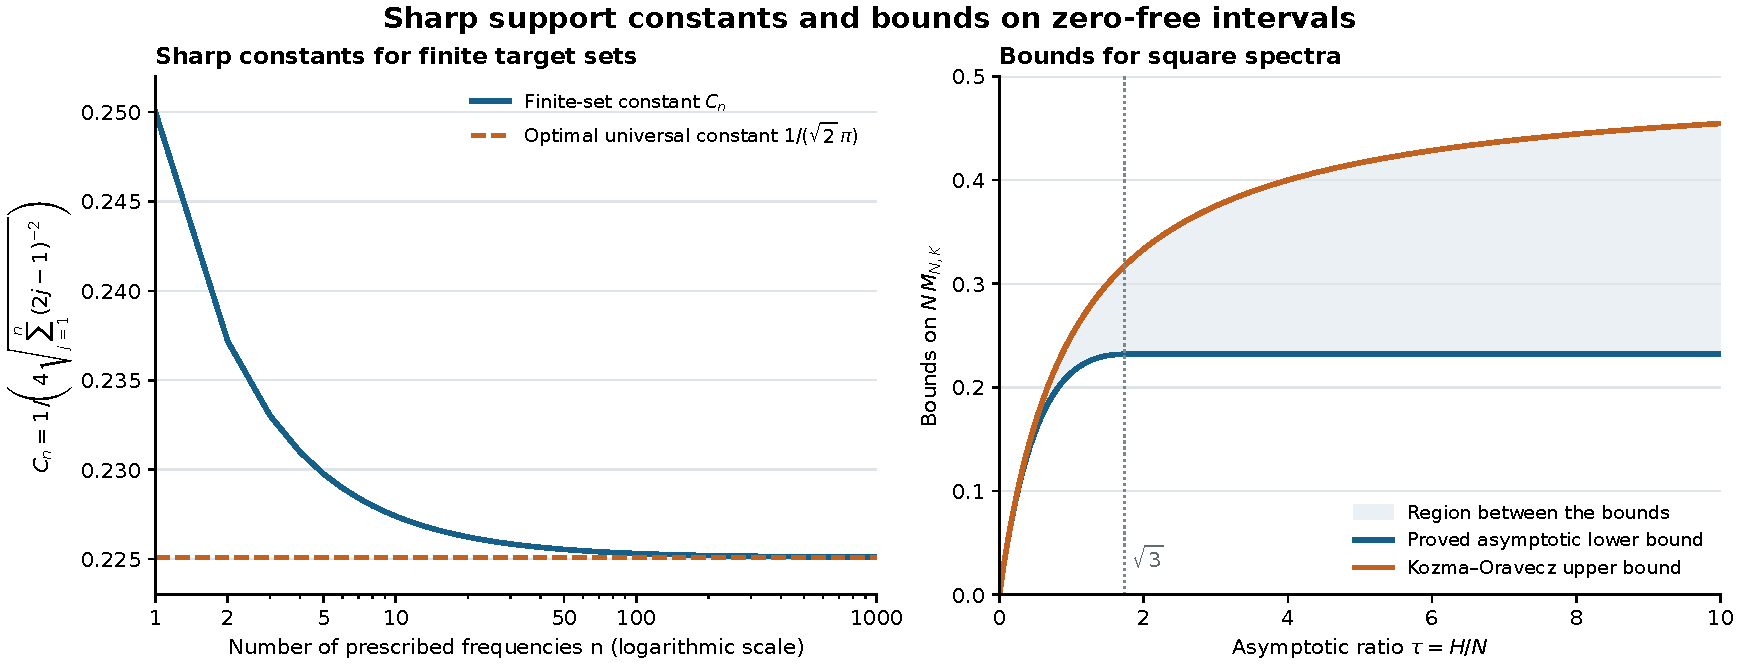
\includegraphics[width=\textwidth]{figures/reciprocal_bounds.pdf}
\caption{Left: the exact finite-cardinality support constants $C_n$ decrease to
$1/(\sqrt2\pi)$. Right: the proved lower and upper bounds in
\eqref{eq:linear}; the region between them is not a numerical computation of the
unknown extremum. The lower curve saturates at $\sqrt3-3/2$.}
\label{fig:bounds}
\end{figure}}{}

\section{An extension to higher powers}

The finite-spectrum inequality also applies without change to higher powers.
Here is a self-contained consequence that needs no regular-variation theory.

\begin{corollary}[Power-frequency tails]\label{cor:powers}
Fix an integer $d\ge2$, and let
\[
 M_{N,H}^{(d)}=M(\{N^d,(N+1)^d,\ldots,(N+H-1)^d\}),\qquad
 M_N^{(d),\infty}=\sup_{H\ge1}M_{N,H}^{(d)}.
\]
Uniformly for $N,H\ge1$,
\[
 M_{N,H}^{(d)}\asymp_d\frac{\min(H,N)}{N^d}.
\]
If $H=o(N)$, then
$M_{N,H}^{(d)}=H(1+O_d(H/N))/(2N^d)$.
Moreover
\begin{equation}\label{eq:powers}
 \sup_{t>0}\frac{(d+1)t^2}{2((1+t)^{d+1}-1)}
 \le\liminf N^{d-1}M_N^{(d),\infty}
 \le\limsup N^{d-1}M_N^{(d),\infty}
 \le\frac1{2(d-1)}.
\end{equation}
The positive maximizing $t=t_d$ in the lower constant is unique and solves
\[
 (1+t)^d\bigl(2-(d-1)t\bigr)=2.
\]
\end{corollary}

\begin{proof}
Use \eqref{eq:general-gaps} with $a_j=(N+j-1)^d$. Taking
$m=\min(H,N)$ gives a lower bound $m/(2(2N)^d)$. The upper bound is at most
$H/(2N^d)$ and at most $\frac12\sum_{n\ge N}n^{-d}=O_d(N^{1-d})$.
This proves the uniform comparison. Uniform expansion within a short band gives
the more precise short-band formula. For $m/N\to t>0$, the scaled prefix bound
tends to $t^2/(2\int_1^{1+t}x^d\dd x)$; integral comparison gives the upper tail
constant in \eqref{eq:powers}. Differentiation gives the displayed critical-point
equation. Its left side starts at $2$, increases until $t=1/(d-1)$, and then
decreases to zero at $2/(d-1)$, since its derivative is
$(d+1)(1+t)^{d-1}(1-(d-1)t)$. Thus exactly one positive crossing of $2$ occurs,
and it is the maximizer.
\end{proof}

\section{Verification and remaining questions}

The proofs above, rather than computation, establish the statements for all
admissible measures and all integer parameters. The accompanying script performs
independent exact-arithmetic checks of the finite-square optimizer, symbolic
identities used in the estimates, and the constants in the support bound. It
also generates the figure. An optional Bernstein-coefficient certificate gives
one concrete square-spectrum polynomial that is positive on a specified interval;
it is illustrative and is not needed for the separation proof.

The manuscript was checked separately for Fourier normalization, multiplicities,
arbitrary real parts of zeros, boundary heights in the strip formula, the
infinite equality argument, the stability restriction to Fourier zeros, and the
distinction between a supremum of zero-free lengths and an attained closed-interval
extremizer. These are mathematical and computational checks, not a Lean
formalization or external peer review.

Several further problems remain precise. Determine the minimum support for a
general prescribed set $A$, beyond the sharp universal inequalities. Determine
whether $N M_N^\infty$ converges and find its value if it does. Improve the
stability constant or determine its optimal deficit exponent. The current
arguments do not resolve these questions, and do not purport to settle a major
conjecture in analytic number theory.

\begin{thebibliography}{9}

\bibitem{ProveIt}
Vladimir Reshetnikov, \emph{ProveIt: Analysis/GeneralizedRiemannHypothesis},
repository snapshot \texttt{41a284d6ef8eb16d783bfc685ab99cc6e1d28daa},
\texttt{Article/sections/fil.tex}, especially labels
\texttt{fil:lem:strip} and \texttt{fil:thm:meanbound}.
\url{https://github.com/VladimirReshetnikov/ProveIt/blob/41a284d6ef8eb16d783bfc685ab99cc6e1d28daa/Analysis/GeneralizedRiemannHypothesis/Article/sections/fil.tex}.
Inspected 27 November 2026, together with the article and available incoming
archives at that snapshot.

\bibitem{EF}
A. Eremenko and A. Fryntov, \emph{Remarks on the Obrechkoff inequality},
Proceedings of the American Mathematical Society \textbf{144} (2016), 703--707.
\url{https://arxiv.org/abs/1409.4849}.

\bibitem{Steinerberger}
S. Steinerberger, \emph{Some Open Problems}, version indexed as last updated
31 March 2026, Problem 41, ``A kind of uncertainty principle?'', p.~41.
\url{https://faculty.washington.edu/steinerb/openproblems.pdf}.
The author's indexed primary text was consulted; direct retrieval of the PDF
returned HTTP 404 during this investigation. An older 10 June 2024 version
numbers the same question 42. The statement used here is recorded explicitly
in Section~4, independently of that numbering.

\bibitem{KO}
G. Kozma and F. Oravecz, \emph{On the gaps between zeros of trigonometric
polynomials}, Real Analysis Exchange \textbf{28} (2002/2003), no.~2, 447--454.
Question 2 in the preprint.
\url{https://arxiv.org/abs/math/0601021}.

\end{thebibliography}
\end{document}
